
\documentclass[12pt]{article}
\usepackage{amssymb,amsmath,natbib,graphicx,amsthm,
  setspace,sectsty,anysize,times,dsfont,enumerate,adjustbox}

\usepackage[svgnames]{xcolor}

\usepackage{lscape,arydshln,relsize,rotating,multirow}
\usepackage{caption}
\captionsetup{%
  font=small,
  labelfont=normalfont,
  singlelinecheck=false,
  justification=justified
}
\usepackage{algorithm}

\marginsize{1.1in}{.9in}{.3in}{1.4in}

\sectionfont{\noindent\normalfont\large\bf}
\subsectionfont{\noindent\normalfont\normalsize\bf}
\subsubsectionfont{\noindent\normalfont\it}

\usepackage[bottom,hang,flushmargin]{footmisc}

\pdfminorversion=4
\begin{document}

\setstretch{1.1} 

\pagestyle{empty}

~
\vskip 2cm

\noindent {\Huge \bf Bayesian and Empirical Bayesian Forests} 

\vskip 2cm

\noindent{\Large Matt Taddy}

{\large
\vskip .25cm \noindent
{The  University of Chicago Booth School of Business}\\
\texttt{faculty.chicagobooth.edu/matt.taddy}}



\vskip 2cm

{\noindent \textbf{Abstract:} We interpret random forests via the framework of
distribution-free nonparametric Bayesian analysis, so that the ensemble
average is an approximation to posterior mean inference for the
population CART tree. This insight motivates a class of fully Bayesian
Forest (BF) algorithms that provide small gains in predictive
performance and large gains in interpretability (from a Bayesian
perspective) over their classically bagged predecessors. The framework
is then applied to derive Empirical Bayesian Forests (EBF), in which a
single short tree ``trunk'' is estimated and Bayesian Forests are fit to
the data at each leaf of the trunk. We are able to derive conditions
under which this fixed trunk has high posterior probability, and
demonstrate that in such settings the EBF performs nearly as well in
out-of-sample prediction as the full BF. The advantage of
pre-partitioning a fixed trunk is that the EBF ensembles can be fit
independently for each initial partition. This implies a novel strategy
for fitting tree ensemble predictors on data stored in a distributed
file system (such as HDFS), and we show that it strongly outperforms the
common strategy of fitting forests to without-replacement data subsets.
The work is illustrated on a number of publicly available examples, and
on massive data from eBay.com.}
 

\newpage
\setstretch{1.5}

\pagestyle{plain}
\vskip 1cm

\section{Introduction}\label{introduction}

Decision trees are a fundamental tool for machine learning. Such trees
partition the attribute (input) space into regions of response
homogenaity, such that the response (output) value associated with any
point in a given region can be predicted from the average of other
observations in that region. The classification and regression tree
(CART) algorithm of Breiman et al (1984) is a common and useful recipe
for building trees; it greedily grows a tree through a series of
partitions on input features, each of which maximizes reduction in some
measure of inpurity at the current tree leaves (terminal nodes; i.e.,
the implied imput space partitioning). The development of \emph{random
forests} (RF) by Brieman in 2001, which predict through the average of
many CART trees fit to bootstrap re-samples of the data, provided an
archetype for the hugely successful strategy of \emph{tree ensemble
learning.} For prediction problems with relatively small input
dimensions (or in conjunction with dimension reduction strategies)
properly trained ensembles of trees -- or forests -- can predict
out-of-the-box as well as any carefully tuned, application-specific
alternative.

This review details a straightforward, but not well-recognized,
nonparametric Bayesian interpretation of random forests. Imagine the
CART fit for a \emph{population} data generating process (DGP) with
finite support. This CART greedily partitions the feature support to
minimize impurity of the response distribtion conditional on each
partition region, and we suppose it terminates while each leaf node has
probability greater than some threshold. If we agree that such a
population-CART is an useful statistic (i.e., would be useful for
prediction) then its posterior mean is of interest as the optimal
Bayesian estimator of a useful statistic. The posterior distribution of
CART fits is induced by our nonparametric Bayesian posterior over random
DGPs. The random forest set of trees is an approximate sample from this
posterior, such that the RF predictor is a \emph{posterior mean}
prediction rule. A simple alteration of the RF algorithm leads to an
exact sample from the posterior, which we label as a \emph{Bayesian
forest}. The altered BF algorithm offers a small but reliable
improvement on RFs. However, the big gain is interpretability: when
should R/B forests work, and when should we expect the more restrictive
Bayesian tree models to be preferable?

The interpretable model also allows us to assess appropriateness of
various Big Data distributed computing schemes for their ability to
recover the posterior mean. From this, we propose Empirical Bayesian
Forests (EBF) in which a single short tree ``trunk'' is estimated and
Bayesian Forests are fit to the data at each leaf of the trunk. We are
able to derive conditions under which this fixed trunk has high
posterior probability, and demonstrate that in such settings the EBF
performs nearly as well in out-of-sample prediction as the full BF. The
advantage of pre-partitioning a fixed trunk is that the EBF ensembles
can be fit independently for each initial partition. This implies a
novel strategy for fitting tree ensemble predictors on data stored in a
distributed file system (such as HDFS), and we show that it strongly
outperforms the common strategy of fitting forests to
without-replacement data subsets. The work is illustrated on a number of
publicly available examples, and on massive data from eBay.com.

    \subsection{Nonparametric Bayesian
Forests}\label{nonparametric-bayesian-forests}

The classical \emph{distribution free} framework of nonparametric
inference \cite{hollander_nonparametric_1999} has two components:
\begin{enumerate}
\item find a \emph{nonparametric statistic} $\mathcal{T}(\text{DGP})$ that is of interest in your application regardless of the true data generating process (DGP),
\item and derive a sampling distribution on $\mathcal{T}$ under minimal assumptions on the DGP.
\end{enumerate}
The Bayesian version of this procedure replaces step 2 with 
\begin{enumerate}
\item[2b.] build a flexible model for the DGP, and derive the posterior distribution on $\mathcal{T}(\text{DGP})$ from the posterior distribution on possible DGPs.
\end{enumerate}
As detailed below, a simple and powerful nonparametric Bayesian framework models the data generating process through a multinomial probability
function on a large number of possible $\mathbf{z} = \{\mathbf{x},y\}$ input-output points. We apply a limiting
non-informative prior, which implies using the observed data as our
approximation for the population support.  This provides a posterior over
possible DGPs.

In the context of this article, 1. is clearly referring to decision trees.   Indeed, trees are useful precisely because they are good predictors regardless of the underlying data distribution -- they do not rely upon distributional assumptions to share information across training observations.  In particular, we'll define $\mathcal{T}$ as the greedy CART fit for a decision tree that terminates at some minimum leaf probability threshold.  For any realization of the DGP -- which will be a probability function over finite support -- the CART tree $\mathcal{T}(\text{DGP})$
greedily splits to minimize impurity of the response distribtion conditional on each partition region.
If we can sample from the posterior over DGPs (i.e., sample weights on the support), then a forest is constructed by fitting CART to each posterior DGP draw.  The forest is a posterior sample of tree statistics, and  the ensemble average prediction is interpretable as a posterior mean.


The forest predictor is a posterior mean for the population CART tree.  This makes it clear when we should expect such forests to do a good job in prediction: when this tree provides a good summary of the conditional response distribution.  This will be the case when the greedy algorithm leads to a good partitioning -- for example, when you have lots of data and a relatively low dimensional feature space.  It will not do as well when the greedy algorithm is unreliable; e.g., in high dimensions, especially when many feature dimensions have little or no influence on the response (i.e., in situations were, even if nonparametric partitioning is the correct approach, the greedy algorithm is likely to converge to a minor mode much worse than best).  More importantly, a forest predictor will also be the inappropriate choice whenever compared against models with properties reflected in the true data generating process.  For example, if the response is a linear function of the features, then knowing the equation for this line through the population is \emph{much more useful} than any partitioning summary.  Or if the idiosynchratic error around the unknown conditional mean function is homoskedastic, we will get better predictions if we use that information when summarizing the conditional response distribution.  The use of Random or Bayesian forests should thus be reserved for situations where we \emph{need} to be distribution free -- when the conditional response function defies parametric representation. 

    \subsubsection{Model for the data generating
process}\label{model-for-the-data-generating-process}

We employ a Dirichlet-multinomial sampling model in nonparametric
Bayesian (NPB) analysis. The approach dates back to
\cite{ferguson_bayesian_1973}. \cite{chamberlain_nonparametric_2003}
provide an overview in the context of econometric problems.
\cite{rubin_bayesian_1981} proposed the Bayesian bootstrap as an
algorithm for sampling from versions of the posterior implied by this
strategy, and the algorithm has since become closely associated with
this model.

Use $\mathbf{z}_i = \{\mathbf{x}_i,y_i\}$ to denote the complete feature
and response observation for unit $i$. We suppose that data are drawn
\emph{independently} from a finite number $L$ of possible values,

\begin{equation}
\mathrm{p}(\mathbf{z}) = \sum_{l=1}^L \omega_l \mathbb{1}{[\mathbf{z} = \boldsymbol{\zeta}_l]}
\end{equation}

where $\omega_l\geq0\forall l$ and $\sum_l \omega_l = 1$. Thus the
generating process for observation $i$ samples $l_i$ from a multinomial
with probability $\omega_{l_i}$, and this indexes one of the $L$ support
points. Since $L$ can be arbitrarily large, and all data are stored as
discrete (up to machine tolerance), this so-far implies no restrictive
assumptions beyond that of independence.

The conjugate prior for $\boldsymbol{\omega}$ is a Dirichlet
distribution, written
$\mathrm{Dir}(\boldsymbol{\omega}; \boldsymbol{\nu}) \propto \prod_{l=1}^L\omega_j^{\nu_l-1}$.
We will parametrize the prior with a single concentration parameter
$\boldsymbol{\nu} = a >0$, such that $\mathbb{E}[\omega_l] = a/La = 1/L$
and $\mathrm{var}(\omega_l) = (L-1)/[L^2(La+1)]$. Suppose you have the
observed sample $\mathbf{Z} = [\mathbf{z}_1 \cdots \mathbf{z}_n]'$. For
convenience, we allow $\boldsymbol{\zeta}_l=\boldsymbol{\zeta}_k$ for
$l \neq k$ in the case of repeated values. Write
$l_1 \dots l_n = 1 \dots n$ so that
$\mathbf{z}_i = \boldsymbol{\zeta}_i$ and
$\mathbf{Z} = [\boldsymbol{\zeta}_1 \cdots \boldsymbol{\zeta}_n]'$. Then
the posterior distribution for $\boldsymbol{\omega}$ has
$\omega_i = a+1$ for $i\leq n$ and $\omega_l = a$ for $l>n$, so that

\begin{equation}
\mathrm{p}(\boldsymbol{\omega} ) \propto \prod_{i=1}^n \omega_i^{a} \prod_{l=n+1}^L \omega_l^{a-1}.
\end{equation}

This, in turn, defines our posterior for the data generating process
through our sampling model above.

There are many possible strategies for specification of $a$ and
$\zeta_l$ for $l>n$. (The unobserved $\zeta_l$ act as data we imagine we
might have seen, to smooth the posterior away from the data we have
actually observed. See \cite{poirier_bayesian_2011} for discussion of
how such values can be useful in application.) The non-informative prior
that arises as $a\rightarrow 0$ is a default with massive computational
convenience: in this limit, $\omega_l = 0$ with probability one for
$l>n$. (To see this, note that for $l>n$ the posterior has
$\mathbb{E}[\omega_l]=0$ with variance
$\mathrm{var}(\omega_l) = \lim_{a \to 0} a[n+a(L-1)]/[(n+La)^2(n+La+1)] = 0$.)
We apply this limiting prior throughout, such that our posterior for the
data generating process is a multinomial draw from the \emph{observed
data points}, with a uniform $\mathrm{Dir}(\boldsymbol{1})$ distribution
on the $\boldsymbol{\omega} = [\omega_1 \dots \omega_n]'$ sampling
probabilities.

    \subsubsection{Posterior inference and Bayesian
forests}\label{posterior-inference-and-bayesian-forests}

Conditional upon $\boldsymbol{\omega}$, the population tree
$\mathcal{T}(\text{DGP})$ is defined through a weighted-sample of the
CART version. In particular, given data
$\mathbf{Z}^\eta = \{\mathbf{X}^\eta,\mathbf{y}^\eta\}$ in node $\eta$,
sort through all dimensions of all observations in $\mathbf{Z}^\eta$ to
find the split that minimizes the average of some $\boldsymbol{\omega}$
impurity metric across the two new child nodes. For example, in the case
of regression trees (which we focus on), the impurity to minimize is
weighted-squared error

\begin{equation}
\mathcal{I}(\mathbf{y}^\eta) = \sum_{i\in \eta} \omega_i (y_i - \bar y^\eta )^2
\end{equation}

with $\bar y^\eta =\omega_i y_i/\|\boldsymbol{\omega}^\eta\|_0$. This is
repeated on every leaf of the tree, and the algorithm terminates when no
split leads to a new child $\|\boldsymbol{\omega}^{\eta^c}\|_0$ with
$\|\boldsymbol{\omega}^{\eta^{c}}\|_0$ greater than some threshold.
We'll refer to the resulting weighted CART as
$\mathcal{T}(\boldsymbol{\omega})$.

Following \cite{rubin_bayesian_1981} we can obtain a sample from the
posterior on $\mathcal{T}(\boldsymbol{\omega})$ through a simple
Bayesian bootstrap: for $b=1,\dots, B$,

\begin{itemize}
\itemsep1pt\parskip0pt\parsep0pt
\item
  draw $\boldsymbol{\omega}^b \sim \mathrm{Exp}(\mathbf{1})$, and set
  $\boldsymbol{\Omega}^b = \mathrm{diag}(\boldsymbol{\omega}^b)$; then
\item
  run CART to get $\mathcal{T}(\boldsymbol{\omega})$
\end{itemize}

We call this a Bayesian Forest, and it differs from a traditional random
forest only in that the weights are drawn from a Dirichlet distribution
rather than a multinomial distribution. To the extent that RF sampling
provides a coarse approximation to the BF samples, the former is a
convenient (and computationally advantageous, since fewer observations
need to be optimized over) approximation.

    \subsubsection{Implementation via
scikit-learn}\label{implementation-via-scikit-learn}

We can implement a BF through simple adjustement of the
\texttt{ensemble} module of \texttt{scikit-learn} (\texttt{sklearn}).
Upon altering the forest \texttt{sample\_counts} when bootsrapping to be
exponential rather than binomial, we get a bayesian bootstrap. We flag
this alternative Bayesian bootstrap by passing \texttt{boostrap=2} in
any forest class construction (this is documented as a boolean, so we're
taking advantage of easy conversion to int).

In detail, lines 88-89 of the \texttt{scikit-learn} \texttt{forest.py} module
change from

\texttt{indices = random\_state.randint(0, n\_samples, n\_samples) sample\_counts = np.bincount(indices, minlength=n\_samples)}

to

\begin{verbatim}
        ### bayesian forest      
        if forest.bootstrap == 2:
            sample_counts = random_state.exponential(1,n_samples)
        else:    
            indices = random_state.randint(0, n_samples, n_samples)
            sample_counts = np.bincount(indices, minlength=n_samples)
        
        #print("bs of %d and first 5 weights:" % forest.bootstrap)
        #print(sample_counts[0:5])
        ###################
\end{verbatim}


    \subsubsection{Motorcycle data
illustration}\label{motorcycle-data-illustration}

We illustrate the various models with a simple one-dimensional
prediction problem: what is the velocity of a motorcyle helmet after
impact in a crash? This data, taken from the MASS library for R,
provides a series of measurements of crash-test-dummy head acceleration
in simulated motorcycle accidents.

\begin{figure}
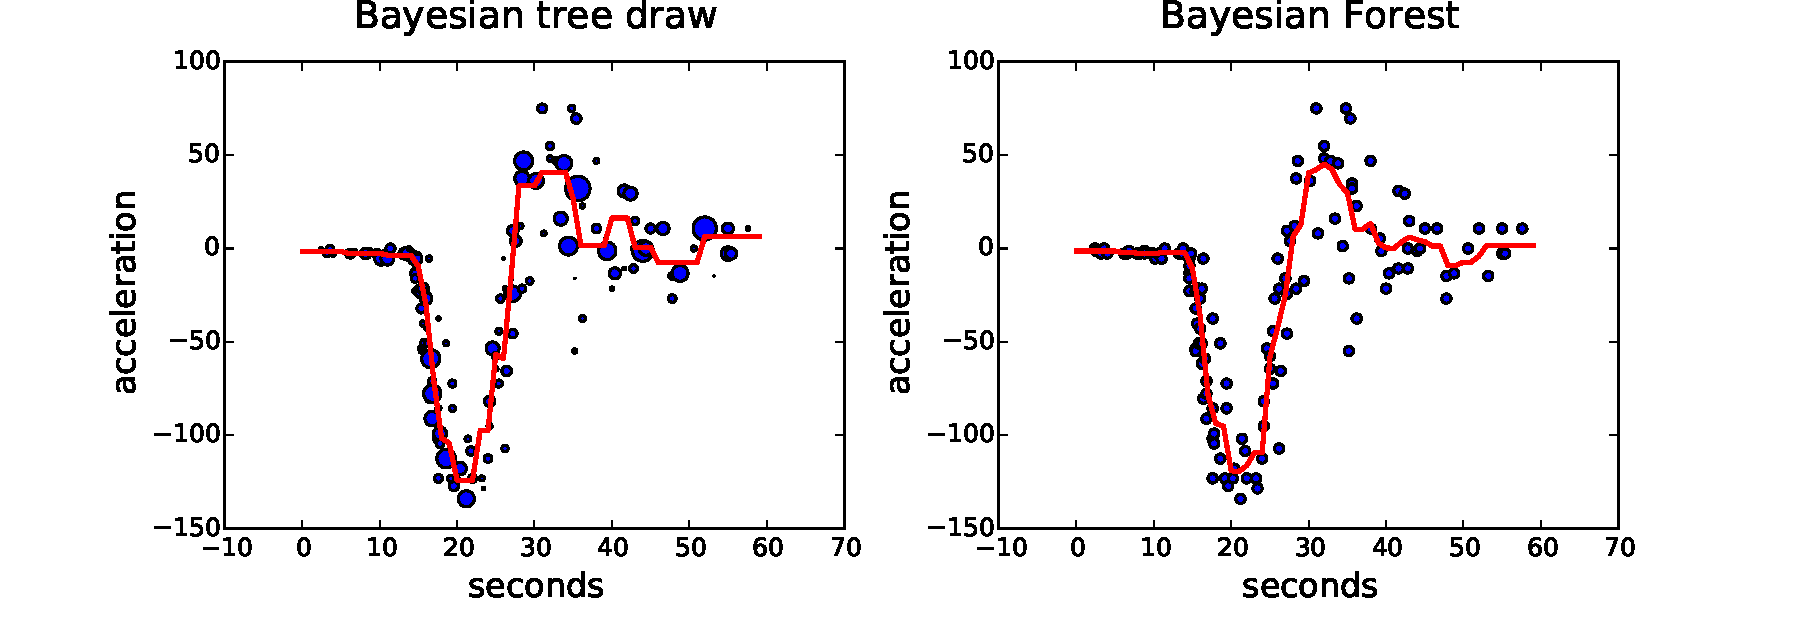
\includegraphics[width=\textwidth]{../graphs/mcycle}    
\end{figure}    

    \subsection{Bayesian tree-as-parameter
models}\label{bayesian-tree-as-parameter-models}

Our multinomial-sampling npB analysis, inspired by classical
distribution-free strategies, can be viewed as a minimal-assumption
baseline Bayesian treatment. There are plenty of other Bayesian analyses
of decision trees in the literature. All of these methods treat the tree
as a \emph{parameter} which governs the DGP, rather than a functional
thereof, and thus place some set of restrictions on the functional form
of the distributional relationship between inputs and outputs. This
section will survey these models and estimators, emphasizing that our
Bayesian Forest framework allows us to place some intuition underneath
the question of when each of these methods will be more appropriate that
the completely nonparametric BF (or RF) baseline.

The original Bayesian tree model is the \emph{Bayesian CART} (BCART) of
Chipman, George, and McCulloch (1998). BCART treats the set of all
possible decision tree fits as the support for their target parameter,
and they devise a prior on trees in this set that has tree probability
decreasing with its complexity (maximum depth and number of node, such
that trees that are equivalent on these properties are equally likely in
the prior). The data model is specified for response $y$
\emph{conditional upon} $\mathbf{x}$, and holds that conditional upon a
given tree the responses for all observations who are allocated (via
$\mathbf{x}$) to the same leaf node are IID from some parametric family.
For regression trees, observations in each leaf node are IID Normal with
shared variance and mean. For classification trees, each leaf represents
single probability function over outcome classes.

BCART is fit through Markov chain Monte Carlo (MCMC). The algorithm
draws a (correlated) posterior sample by proposing a number of possible
changes to existing tree fit (e.g.~grow or prune a given leaf node in
the current tree) and accepting those changes (and thus move to new
posterior tree draw) with probabilities proportional to the tree prior
times leaf likelihood. A natural extension of this framework is to
consider alternative leaf models. The original BART authors proposed
linear regression at leaves, while the Treed Gaussian Processes of
\cite{gramacy_bayesian_2008} use Gaussian procees regression at each
leaf node. The TGP models, in particular, are very appealing in that
they use the tree structure (one flexible regression model) to allow for
nonstationarity in the Gaussian processes (another flexible regression
model). As an alternative to MCMC-based tree frameworks,
\cite{taddy_dynamic_2011} proposed dynamic regression trees (dynaTree)
fit through sequential Monte Carlo (SMC). In particular, dynaTree uses a
particle-filtering to sequentially update a particle set of potential
trees for the arrival of new data with basic (grow, prune) tree
operations -- they allow the tree to grow naturally with streaming data.

MCMC and SMC seem naturally suited to analysis of CART, as their
sampling of tree space relies upon the same incremental moves that are
familiar from the construction of classical CART fits. However, this
also means that these sampling algorithms are subject to the same
\emph{problems} CART has: they tend to get stuck in small regions of
tree-space. For dynaTree SMC, the quality of the particle set degrades
quickly (although for truly streaming data, particle rejuvination can
help dramatically and has the secondary benefit of allowing tree
structure to change in time). The issue is alleviated by having more
complex leaf models, as in TGP, since then shorter (easier to sample
efficiently) trees are required for fitting the data. Standard Monte
Carlo algorithm enhancements, such as multiple parallel chains, can also
help. But a full exploration of BCART-style tree space remains very
difficult and requires extremely large Markov samples to have any chance
of convergence.

As a solution to these mixing issues, the original BCART authors
proposed Bayesian Additive Regression Trees \cite{chipman_bart:_2010},
which replaces the single tree model with the sum of many small trees.
Thus, a single observation is allocated via its features to a leaf node
in each of, say, $T$ trees; the associated response is then distributed
with mean equal to the average of each leaf node value and with a
\emph{shared variance across observations}. The original BART model
assumes Normal response, and later extensions allow alternative response
families (including nonparametric mixtures of Normals). BART solves the
mixing issue by only working with very short (depth 2-5) trees. This
stubby tree space is not difficult to explore, and the authors provide a
fast and well-mixing MCMC algorithm. However, this resolution comes at a
steep price: by specifying a data model that has shared variance for all
observations, BART loses an important feature of CART, BCART, and the
others: the ability to fit fitting heteroskedastic data. While the other
BCART-style Bayesian trees made assumptions about the parametric
distribution at each leaf node, they all (as CART does) allow completely
different specifications (e.g., distinct mean and variance) at each
leaf. BART's shared variance removes this property.

Despite the assumed homoskedasticity, extensive simulations have shown
BART to outperform alternative flexible prediction rules. The empirical
evidence of BARTS performance is strong enough that it has gained
support as a default Bayesian method for flexible prediction
\cite{hill_bayesian_2011}. From our perspective, this success occurs
when an estimate of the BART model on the population, with its
homoskedastic Normal error variance, is a good summary of the population
conditional response distribution. Many datasets, especially those
analyzed by academics (and after the transformations, e.g., log, that
academic statisticians apply to get better behaved response), have the
property that they are well fit by flexible regression with
homoskedastic errors. For the same reasons, the BCART/TGP/dynaTree
models have been shown repeatedly to outperform RF in academic
bake-offs; this occurs on data were their parametric response model
(e.g.~Normal) fits well enough to be a better summary of the data than
the posterior mean CART tree. The purpose of the current article is not
at all to argue against such strong performance. Rather, we wish to add
intuition about the models that would allow you to consider your data
applications and predict, given some basic knowledge of the DGP, whether
you can leverage any of the semiparametric assumptions in BART, BCART,
TGP, dynaTree, etc; or whether a distribution free summary (BF or RF)
will be more useful.

Finally, we note that the Bayesian bootstrap framework can also applied
to parameters of an assumed parametric DGP, and thus can apply to
tree-as-parameter models. In such a framework, outlined as Bayesian
bagging in \cite{clyde_bagging_2001}, the bootstrap mean (and related
bootstrap summaries) have interpretation as \emph{Bayesian model
averaging}. However, this framework becomes difficult to interpret when
the target parameter is infinite dimensional (as it is for tree models),
and the MCMC or SMC sampling strategies mentioned above are much more
common. The Clyde+Lee paper does consider a Bayesian bagging (model
averaging) treatment of CART, but their desire to interpret the tree as
a model parameter leads to quite different algorithm and analysis.

    \subsection{Compare and contrast}\label{compare-and-contrast}

The spectrum of Bayesian analysis of trees moves from distribution free
BF and RF, through the Bayesian nonparametrics-via-many-parameters
approach of BCART, TGP, and dynaTree, to semi-parametric BART which
makes truly restrictive assumptions about the response distribution.
Instead of blindly picking the method which has performed best in past
studies of arbitrary data (e.g., bake-offs in academic papers), we can
use this information to predict which methods will suit our application.

In this section, we illustrate with two examples that have very
different properties. The first is a simulation study with known
homoskedastic errors in the target. The second considers raw
dollar-value home prices in california as the response of interest. On
these examples, we fit a CART, RF, BF, BART, and BCART as described
above. We also include the extremely random trees (ET) of
\cite{geurts_extremely_2006}, which are similar to random forests except
that (a) instead of optimizing greedy splits, candidate splits are
chosen randomly and the best is used and (b) all of the data is used to
fit each tree (there is no bootstrap resampling or reweighting). ETs
perform well on small datasets, where CART has a high tendancy to
overfit without careful pruning. On such small datasets (e.g.~our
Friedman example) the restriction of population support to observed
support (assumed in our nonparametric analysis) becomes less acceptable
and we might expect the Random and Bayesian forests to suffer.

\subsubsection{Friedman example}\label{friedman-example}

A common simulation experiment in evaluating flexible predictors is
based around the so-called Friedman function, first proposed for this
purpose in \cite{friedman_multivariate_1991} MARS paper. The function is

\[
y = f(\mathbf{x}) +  \varepsilon = 10\mathrm{sin}(\pi x_1 x_2) + 20 (x_3-0.5)^2 + 10x_4 + 5x_5 + \varepsilon
\]

where $\varepsilon \sim \mathrm{N}(0,1)$ and $x_j \sim \mathrm{U}(0,1)$.
We include as features for training the spurrious $x_6 \dots x_{p}$,
matching Friedman with MARS and Chipman et al with BART. Each candidate
regression model is fit to 100 random draws from the Friedman function,
and tested at 1000 new x locations (simulated uniformly as in the
training data). We calculate the root mean square error between
predicted values and true $f(\mathbf{x})$ as a measure predictive
performance.

   
    \begin{center}
    \adjustimage{max size={0.9\linewidth}{0.9\paperheight}}{bayesforest_files/bayesforest_16_1.png}
    \end{center}
    { \hspace*{\fill} \\}
    

    \begin{verbatim}
        bart     1.811829
        ET       2.609423
        BF       2.670613
        RF       2.743355
        DT       3.771928
        bcart    3.910470
\end{verbatim}
        
    \begin{center}
    \adjustimage{max size={0.9\linewidth}{0.9\paperheight}}{bayesforest_files/bayesforest_19_1.png}
    \end{center}
    { \hspace*{\fill} \\}
    
    As predicted, the only model that assumes the (true) homoskedastic error
structure, BART, well outperforms all others. The two forests, BF and
RF, are both a large improvement over a single decision tree. The fully
Bayesian BF is only about 1\% better than the approximately Bayesian RF,
as Bayesian and classical bootstrapping weights differ little in
practice. Both are outperformed slightly by the extremely random trees
(ET), which might be expected due to the small sample size (for which
the observed support approximation to population support, assumed in our
forest interpretation, is poor). The only suprise for us is the very
poor performance of BCART (even worse than a single decision tree); we
hypothesis that this is due to the notoriously poor mixing of the BCART
MCMC, such that this fit is neither finding a posterior mean (as it is
intended to) or optimizing to a local posterior mode (as DT does).

    \subsubsection{California housing data}\label{california-housing-data}

For the next example, we consider prediction of median home price by
census block in california, based upon eight features of each region
(location, income, housing stock). The data are taken from
http://www.dcc.fc.up.pt/\textasciitilde{}ltorgo/Regression/cal\_housing.html.
This problem has a response distribution that is difficult to summarize
parametrically. Standard analysis takes the log price as the response of
interest, which at least tames some of the error heteroskedasticity.
Instead, we will attempt to model the conditional expection of raw
dollar home values. This mimics the setting common in the analysis of
online transaction data (e.g.~clicks or dollars spent), where the
variable average effects and predictive performance on raw \$ or click
scale are of primary interest.


    \begin{center}
    \adjustimage{max size={0.9\linewidth}{0.9\paperheight}}{bayesforest_files/bayesforest_22_1.png}
    \end{center}
    { \hspace*{\fill} \\}
    
    It appears from the histogram (and investigating the raw values) that
the data has been capped at 500k. In any case, the unconditional
response has a long right tail, but is much more regular than what we
commonly see in digital commerce applications (e.g., see Taddy et al,
2014, for transaction data with massive spikes at zero and at
psychological price thresholds, as well as a tail that includes values
50k times larger than the mean).


    Note that bart fit takes around 75 sec in R, vs 10 sec for BF run in
serial.


    \begin{verbatim}
bart-BF: 0.130740872538
ET-BF: 0.0834811139448
RF-BF: 0.00350375895282
    \end{verbatim}

            \begin{verbatim}
         BF       48423.638310
         RF       48593.303066
         ET       52466.097577
         bart     54754.587034
         DT       65514.564877
         bcart    82695.262723
         dtype: float64
\end{verbatim}
        
    \begin{center}
    \adjustimage{max size={0.9\linewidth}{0.9\paperheight}}{bayesforest_files/bayesforest_27_2.png}
    \end{center}
    { \hspace*{\fill} \\}
    
    The results are now reversed (except for DT and BCART, which still
underperform all others). The methods which place no assumptions on the
data generating process, RF and BF, do much better than BART and it's
restrictive error model. The implicit regularization of extratrees is no
longer of any benefit, as the larger sample size means that our finite
support approximation is solid. As always, BF offers a real but small
gain over RF.

    \subsection{Empirical Bayesian
Forests}\label{empirical-bayesian-forests}

The previous sections re-interpret forests (random or Bayesian -- they
are roughly equivalent) as samples from the distribution-free posterior
over greedy CART fits. This interpretation is now applied to guide
strategies for forest fit on massive data, by treating that problem as
one of \emph{approximate} sampling from the posterior.

\emph{Empirical Bayes} (EB) is an established framework with a
successful track record in fast approximate Bayesian inference; see,
e.g., \cite{efron_large-scale_2010} for an overview. In parametric
models, EB can be interpreted as fixing at their marginal posterior
maximum (MAP) the parameters at higher levels of a \emph{hierarchical
model}. For example, in the simple setting of many group means (the
average student test score for each of many schools) shrunk to an
overall global center (the outcome for an imaginary `average school'),
an EB procedure would first find the overall average test score across
all schools and then shrink posterior estimated score means towards this
value within each individual school. \cite{kass_approximate_1989}
investigate such procedures and show that, under fairly general
conditions, the conditional posterior (conditioning on a marginal MAP
overall average) for each group mean (school score average) quickly
approaches the fully Bayesian unconditional posterior as the sample size
grows.

CART trees are not a parametric model, but they are hierarchical and
admit an interpretation similar to those studied in
\cite{kass_approximate_1989}. The data which reaches any given interior
node is a function of the partitioning implied by nodes shallower in the
tree. Moreover, due to the \emph{greedy} algorithm through which CART
grows, a given shallow tree is unaffected by changes to the tree
structure below. Finally (this point is investigated in detail in the
next section), the partitioning implied by shallower sub-trees is much
more stable (has lower posterior variability) than the fully grown
trees.

An Empirical Baysian Forest (EBF) takes advantage of this hierarchical
struture by fixing the highest levels in the hierarchy -- the earliest
CART splits -- at a single estimate of high posterior probability. We
refer to this fixed sub tree as the \emph{trunk}, and will generally
take it as a large-leaf (i.e., short) CART fit to the entire dataset.
This is fit to unweighted data, which corresponds to the mean of our
nonparametric Bayesian posterior over DGPs. Based upon this trunk, data
is partitioned into leaves of manageable size, and a forest is fit to
each. That is, EBF replaces the BF posterior sample of trees with a
conditional posterior sample that takes the pre-fit trunk as fixed at
its marginal MAP. Since this trunk has relatively low variance, the EBF
should provide predictions similar to that of the full BF.

EBF is contrasted to a common existing algorithm, which for Big Data
simply splits the data into sub-samples and fits a forest to each
(cite?). This strategy can be justified from standard sampling theory as
yeilding a tree average that is unbiased for the population tree
average, but it discards information available in the full Big Data
sample. Given the high uncertainty and low effective sample sizes
associated with deep tree structure (otherwise, we wouldn't need to
bother with Big Data in the first place), such sub-sampling is ignoring
potentially useful information. Indeed, the next section argues that so
long as the initial tree Trunk is not overfit, then EBF should
outperform forest fits averaged across data subsets. Either approach can
be used in conjuntion with further techniques for distribution of the
tree fit, e.g.~via the PLANET MapReduce scheme of
\cite{panda_planet:_2009}.

    \subsubsection{Uncertainty about trees}\label{uncertainty-about-trees}

Theory on decision trees is sparse. The original CART book of
\cite{breiman_classification_1984} provides results on the consistency
of tree partitioners; they show that any partitioner that which is able
to eventually learn enough to partition into very small-diameter leaves
relative to the DGP probability function will be able to reproduce the
conditional response distribution of that DGP. However, this result says
little about the structure of the underlying trees, nor does it say
little about the ability of a tree to predict when there is not enough
data to reproduce a finely partition the DGP. Another set of theory
focuses on the frequentist properties of individual split decisions. In
the original CHAID work of \cite{kass_exploratory_1980}, split decisions
(on soley categorical variables) are based upon $\chi^2$ tests of the
contingency table at each leaf node. \cite{loh_regression_2002} and
\cite{hothorn_unbiased_2006} are example generalizations, both of which
combat the various multiple testing and other biases inherrent in
tree-building through a sequence of hypothesis tests. However, such
contributions provide little intuition about the variability of an
entire decision tree or in the setting where we are not working from a
no-split null hypothesis distribution.

Despite this lack of theory, it is widely recognized that there is a
large amount of uncertainty (sampling, or posterior) about the structure
of decision trees. For example, \cite{geurts_investigation_2000} present
a large amount of simulation-based empirical evidence of tree
uncertainty, and they find that the locations and order of split points
in trees is sometimes no-better than random (indeed, this motivates work
by the same authors on extremely random trees). The intuition behind
such randomness is clear: the probability of a tree having any given
branch structure is the product of conditional probabilities for each
successive split. After a enough steps any specific tree approaches
probability of zero. This uncertainty argues for the inherrently `Big'
data requirements of flexible tree regression: there is enough model
complexity and uncertainty that we need to bring as much data as
possible to bear on learning. This was observed by, e.g., the authors of
\cite{panda_planet:_2009} when they compare RFs fit to the full dataset
to those averaged across tree fits on without-replacement sub-samples of
the data (which is a common technique for fitting RFs in distribution).

However, it is possible that elements of the tree structure are
relatively stable. For example, in the context of boosting,
\cite{appel_quickly_2013} argue that the \emph{conditionally} optimal
split locations for internal nodes (they call stumps) are learnable from
subsets of the full data alocated to each node. They use this to propose
a faster boosting algorithm. In this paper we make a related claim: the
top of a tree (its trunk) has structure that is stable enough that it
can be estimated in advance and fixed at a posterior mode. Our argument
for the potential stability of tree trunks begins with a result on the
mean and variance of the difference, at each internal node, betwen MSE
associated with the modal CART partioning and the MSE that results after
a split at any other location. The uncertainty associated with these
statistics, the maximum of which determines our tree, is shown to shrink
with $e^{-n}$ under our npB model. This is reasurring. Moreover, we can
lower bound the probability of selecting the modal CART split among $p$
possible as $1 - \frac{p}{\sqrt{n}} e^{-n}$, which will be quickly close
to one even if $p$ grows with $n$.

    \subsubsection{Probability of the sample CART
tree}\label{probability-of-the-sample-cart-tree}

We focus on regression trees for this example, wherein node impurity is
measured as the sum of squared errors. Consider the simplified setup
where each $x_j \in \{0,1\}$ is a binary random variable (possibly
created as a discretization of a continuous input or through dummy
expansion of a categorical input). Say that
$\texttt{f}_j=\{i:x_{ij}=0\}$ and $\texttt{t}_j=\{i:x_{ij}=1\}$ are the
corresponding implied partitions. We will derive the distribution for
the weighted SSE resulting from a split on any such variable,

\[
\sigma^2_j(\boldsymbol{\theta}) = \frac{1}{n}\sum_i \theta_i \left[y_i - \mu_j(x_{ij})\right]^2
\]

where
$\mu_j(0) = \sum_{i \in \texttt{f}_j}y_i \,\theta_i/\left|\boldsymbol{\theta}_{\texttt{f}_j}\right|$
and
$\mu_j(1) = \sum_{i \in \texttt{t}_j}y_i \,\theta_i/\left|\boldsymbol{\theta}_{\texttt{t}_j}\right|$.

We can simulate the posterior for $\sigma_j$ implied by the gamma
posterior on weights $\boldsymbol{\theta}$, but an exact analytic
expression is not available. Instead, we follow the approach used in
\cite{lancaster_note_2003}, \cite{poirier_bayesian_2011}, and
\cite{taddy_heterogeneous_2014}: we derive a first-order Taylor
approximation to the function $\sigma_j$ and describe the posterior for
that related functional. In particular, the $1\times n$ gradient of
$\sigma_j$ with respect to $\boldsymbol{\theta}$ is

\begin{align}
\nabla \sigma^2_j & = \nabla  \frac{1}{n}\left[\sum_i \theta_iy_i^2 - \frac{1}{\left|\boldsymbol{\theta}_{\texttt{f}}\right|}\left(\mathbf{y}_{\texttt{f}}'\boldsymbol{\theta}_{\texttt{f}}\right)^2
- \frac{1}{\left|\boldsymbol{\theta}_{\texttt{t}}\right|}\left(\mathbf{y}_{\texttt{t}}'\boldsymbol{\theta}_{\texttt{t}}\right)^2\right]
\end{align}

which has elements $ \nabla_{i} \sigma^2_j = \left(y_i -
\mu(x_{ij})\right)^2/n $

The Taylor approximation is then \[
\sigma^2_j \approx \tilde\sigma^2_j  = \sigma^2_j(\boldsymbol{1}) + \nabla \sigma^2\big |_{\boldsymbol{\theta}=\mathbf{1}} (\boldsymbol{\theta} - \boldsymbol{1}) =  \frac{1}{n}\sum_i \theta_i \left(y_i - \bar{y}_j(x_{ij})\right)^2
\] with
$\bar y_j(0) = \frac{1}{n_{\texttt{f}_j}}\sum_{i \in \texttt{f}_j}y_i$
and
$\bar y_j(t) = \frac{1}{n_{\texttt{t}_j}}\sum_{i \in \texttt{t}_j}y_i$
are the observed response averages in each partition.

    Suppose that
$\sigma_1(\boldsymbol{1}) < \sigma_j(\boldsymbol{1})~\forall j$, so that
variable 1 is that selected to dictate partitioning by CART. Then we can
consider variability about this selection by looking at the difference
betwen the approximate SSE for alternative partitions and this modal
value,

\[
\Delta_j(\boldsymbol{\theta}) = \tilde\sigma_1^2 - \tilde\sigma_j^2 =  \frac{1}{n}\sum_i \theta_i
\left[\bar{y}_1^2(x_{i1})-\bar{y}^2_j(x_{ij}) - 2y_i\left(\bar{y}_1(x_{i1})-\bar{y}_j(x_{ij})\right)\right] \equiv \frac{1}{n}\sum_i \theta_i d_{ji}.
\]

Say $\mathbf{d}_j = [d_{j1}\ldots d_{jn}]'$ is the vector of squared
error differences. Then the total difference has mean
$\mathbb{E}\Delta_j  = \bar{d}_j$ and variance
$\mathrm{var}\Delta_j =  \mathbf{d}_j'\mathbf{d}_j/n^2$. Since
$\Delta_j$ is the mean of independent Gamma random variables with known
means and variances, the central limit theorem applies so that delta
converges in distribution to a Gaussian

\[
\sqrt{n}(\Delta_j(\boldsymbol{\theta}) -\bar{d}_j)\rightsquigarrow \mathrm{N}(0,~\mathbf{d}_j'\mathbf{d}_j/n ).
\]

Thus the full-sample CART split occurs if all $\Delta_j< 0 $, which
occurs with probability (note $\bar d_j < 0$)

\[
\mathrm{p}\left(\Delta_j< 0 :~ j = 2\dots p \right) \geq 1 - \sum_{j=2}^p \mathrm{p}( \Delta_j > 0 )\rightsquigarrow 1 
 - \sum_{j=2}^p \Phi\left( -\frac{\sqrt{n}\left|\bar{d}_j\right|}{\sqrt{\mathbf{d}_j'\mathbf{d}_j/n}}\right) 
 \geq 1 -  \frac{1}{\sqrt{2\pi}} \sum_{j=2}^p \frac{\exp(-n z^2_j/2)}{z_j\sqrt{n}} 
\]

where
$z_j = \left|\bar{d}_j\right|\left(\mathbf{d}_j'\mathbf{d}_j/n\right)^{-\frac{1}{2}}$
is sample mean increase in impurity over the sample standard deviation
of impurity. This ratio is bounded in probability, so that that the
exponential bound goes to zero very quickly with $n$. In particular,
ignoring variation in $z_j$ across variables we get

\[
\mathrm{p}\left(\text{split matches sample CART}\right) \gtrsim 1 - \frac{p}{\sqrt{n}} e^{-n}.
\]

Thus, even in a more difficult setting where $p \approx n\times d$, with
$d$ some underlying continuous variable dimension and $p$ the input
dimension discretization on these variables, the probability of the
observed split goes to one at order $\mathcal{O}(n^{-1})$ if
$d < e^{n}/n^{3/2}$.

Given this, why is there any uncertainty at all about trees? The answer
is recursion: each split is conditionally stable given the sample at the
current node, but the probability of any specific sequence of splits is
roughly (we don't actually have independence) the product of individual
node split probabilities. This can get small as we move deeper down the
tree. Moreover, given one split different from the sample CART tree, the
rest of the tree will grow aribitrarily far from this modal structure.
In addition, the sample size going into our probability bounds is
shrinking exponentially with each partition, whereas the dimension of
elligible split variables is reduced only by one at each level.

\subsubsection{tree stability in california}\label{tree-stability-in-california}

We'll illustrate trunk stability and the idea of EBFs on the California
housing data from above. To begin, consider a \emph{trunk} with no less
than 3500 census blocks (out of 20640 total) in each leaf partition.
Greedy CART leads to a five node tree.

    
    \begin{center}
    \adjustimage{max size={0.9\linewidth}{0.9\paperheight}}{bayesforest_files/bayesforest_35_0.png}
    \end{center}
    { \hspace*{\fill} \\}
    

    \paragraph{Shallow tree variance}\label{shallow-tree-variance}

The tree above represents the optimal (greedy) five partition CART. As
predicted by theory, it turns out to be very stable. Running a random
forest of trees which stop at this minimum leaf size, we get


    \begin{verbatim}
freq of CART tree ['medianIncome', 'medianIncome', 'latitude', 'housingMedianAge']: 69
freq of  tree ['medianIncome', 'medianIncome', 'latitude', 'medianIncome']: 18
freq of  tree ['medianIncome', 'medianIncome', 'medianIncome']: 5
freq of  tree ['medianIncome', 'medianIncome', 'medianIncome', 'housingMedianAge']: 3
freq of  tree ['medianIncome', 'medianIncome', 'housingMedianAge']: 3
freq of first three ['medianIncome', 'medianIncome', 'latitude']: 88
freq of first two ['medianIncome', 'medianIncome']: 100
freq of any split on latitude: 88
freq of any split on housingMedianAge: 75
    \end{verbatim}
        
    \begin{center}
    \adjustimage{max size={0.9\linewidth}{0.9\paperheight}}{bayesforest_files/bayesforest_39_1.png}
    \end{center}
    { \hspace*{\fill} \\}
    
    We can also repeatedly sample 90\% of the data, and the CART fit with
\texttt{min\_sample\_leaf=3500} is always similar: from visual
inspection, each fold fit splits on the same variables, just on slightly
different values. Moreover, a Bayesian forest of trees limited to this
node size does little better in OOS prediction (only 1\%), offering
additional evidence that the single CART fit is close to the posterior
mean at this depth.
        
    \begin{center}
    \adjustimage{max size={0.9\linewidth}{0.9\paperheight}}{bayesforest_files/bayesforest_41_1.png}
    \end{center}
    { \hspace*{\fill} \\}
    
    \paragraph{OOS experiment}\label{oos-experiment}

Finally, we consider OOS prediction for the EBF, using a trunk fixed at
the shallow trees from above, and averaging of Bayesian forests fit to
sub-samples of comparable size. The EBF does around 8\% better than
random sub-sampling, and only around 2\% worse than the BF fit to the
entire dataset.


    \begin{verbatim}
2.0\% worse than full sample BF
8.0\% better than random sub sampling
    \end{verbatim}

    \begin{center}
    \adjustimage{max size={0.9\linewidth}{0.9\paperheight}}{bayesforest_files/bayesforest_45_1.png}
    \end{center}
    { \hspace*{\fill} \\}
    
    \subsubsection{Another example: wine
quality}\label{another-example-wine-quality}

As another test of OOS performance, we consider the Vino Verde dataset
of http://www3.dsi.uminho.pt/pcortez/wine/. There are 4898 observations
on 11 continuous attributes (physiochemical properties of the wine) plus
wine color (red or white) as inputs, with an `expert' quality ranking on
the scale of 0-10 as response. Here, we find that averaging forests fit
to 5 random subsets of the data do 10\% worse in OOS prediction than the
EBF conditional on pre-tree partitioning into 5 leaves. Here, the EBF
does close to as well as a full forest: it is only 1\% more expensive
than the full BF fit.

       
    \begin{center}
    \adjustimage{max size={0.9\linewidth}{0.9\paperheight}}{bayesforest_files/bayesforest_47_2.png}
    \end{center}
    { \hspace*{\fill} \\}

    \begin{verbatim}
1.0\% worse than full sample BF
10.0\% better than random sub sampling
    \end{verbatim}

    \begin{center}
    \adjustimage{max size={0.9\linewidth}{0.9\paperheight}}{bayesforest_files/bayesforest_49_1.png}
    \end{center}
    { \hspace*{\fill} \\}
    
    \subsection{Discussion}\label{discussion}

Tree-based learning algorithms are massively useful and very popular.
However, the lack of parametric structure makes it difficult to find
meaningful theoretical guidance for their performance in different
settings. This leads to an exclusive reliance upon cross validation
experiments (and simulation studies) for evaluating candidate
algorithms, which while informative is less helpful for a practitioner
who needs to know which algorithm is best suited to particular data.
Bayesian modelling and interpretation of tree models is a help here, as
the model assumptions and properties are transparent to anyone who is
able to understand probabalistic models. Our Bayesian Forests bring this
intuition to one of the most heavily used tree-based algorithms, Random
Forests, and thus allow it to be realated easily to other candidate
Bayesian methods.

The other contribution here, which likely has more practical
implications, is the proposal of Empirical Bayesian forests. Given our
Baysian interpretation of Forests, the common idea of fixing high-level
parameters with little uncertainty is applied in an algorithm that
yields posterior mean predictions close to that of a forest fit to the
full dataset while working efficiently on small sub-samples. Even if one
is not willing to assume in advance how deep a tree will be stable, in
environments where forests are repeatedly re-fit (to incorporate
incomming information) one can monitor the stability at higher levels
and use this information to fix some tree elements in future runs. This
type of strategy is the key to efficient machine learning on Big Data:
focus the use of massive samples on the pieces of models that are most
difficult to estimate.

\setstretch{1}\small
\bibliographystyle{chicago}
\bibliography{ipython}

    
    \end{document}
